\iftoggle{title}{
\subsection*{Problem 1}
}{}
\iftoggle{contributions}{
\textit{Created by Tyler Wilson 2023}
}{}

\iftoggle{difficulty}{
Difficulty: $\medblackstar \medblackstar \medwhitestar$
}{}

A $16\units{cm}$ long wire of charge $Q=40\units{\mu C}$ is bent into a square in the xy-plane.

\begin{center}
\begin{tikzpicture}
    \draw (-2,-2) -- (2,-2) -- (2,2) -- (-2,2) -- (-2,-2);
    \node[below] at (0,-2) {$4\units{cm}$};
    \draw[fill=black] (0,0) circle (0.05) node[below, left] {0};
    \draw[dashed, ->] (0,0) -- (0,3) node[right] {$y$};
    \draw[dashed, ->] (0,0) -- (3,0) node[right] {$x$};
\end{tikzpicture}
\end{center}

\begin{enumerate}
    \item Find the electric field strength $20\units{cm}$ vertically above the center of the square.
\end{enumerate}
A point charge of mass $m=100\units{g}$ and charge $-5\units{\mu C}$ is now placed at a height $z=20\units{cm}$ above the center of the square.
\begin{center}
\begin{tikzpicture}
    \draw (-2,0) -- (2,0) node[midway, below] {0};
    \draw[dashed] (0,0) -- (0,2) node[midway, right] {$z$};
    \draw[fill=red] (0,2) circle (0.1) node[above, right] {$q=-5\units{\mu C}$};
\end{tikzpicture}
\end{center}
\begin{enumerate}
    \setcounter{enumi}{1}
    \item Find the magnitude and direction of the force acting on the point charge initially when $z=20\units{cm}$.\\
    (Either draw the direction of the force or use vector notation to specify the direction.)
    \item Plot the acceleration of the point charge as a function of it's distance $z$ above the center of the square.
\end{enumerate}

\iftoggle{solutions}{
\textbf{Solution:}
\begin{enumerate}
    \item We can break this problem down into the simpler problem of computing the electric field due to a straight piece of wire. We can then use the superposition principle to find the electric field due to the square.\\
    Electric field due to a straight piece of wire of length $a$:
    \begin{center}
    \begin{tikzpicture}
        \draw[thick] (-4,0) -- (4,0);
        \node[below] at (-2,-0.2) {$a/2$};
        \node[below] at (2,-0.2) {$a/2$};
        \draw[dashed] (-2,0) -- (0,2) -- (0,0);
        \draw[->,red] (0,2) -- (1,3);
        \draw[->,blue] (0,2) -- (1,2);
        \draw[->,blue] (0,2) -- (0,3);
        \node[red, right] at (1,3) {$\vec{E}$};
        \node[blue, above] at (0,3) {$E_z$};
        \node[blue, below] at (1,2) {$E_x$};
        \node[right] at (0,1) {$z$};
        \node[above] at (-1,1.2) {$r$};
        \node[above] at (-0.6,0) {$x$};
        \draw (-2,0) ++(0:0.5) arc (0:45:0.5);
        \node[right] at (-1.5, 0.25) {$\theta$};
    \end{tikzpicture}
    \end{center}
    \begin{align*}
        &d\vec{E}=\frac{1}{4\pi\epsilon_0}\frac{dq}{r^2}\hat{r}\\
        &dq=\lambda dx\\
        &r=\sqrt{x^2+z^2}\\
        &\vec{E}=\int d\vec{E}=\int_{-a/2}^{a/2}\frac{1}{4\pi\epsilon_0}\frac{\lambda dx}{x^2+z^2}\hat{r}\\
        &\vec{E}=\frac{\lambda}{4\pi\epsilon_0}\int_{-a/2}^{a/2}\frac{dx}{x^2+z^2}\hat{r}\\
    \end{align*}
    Note that because of symmetry on each side the electric field will only have a vertical component.
    \begin{align*}
        &\hat{r}=\cos(\theta)\hat{x}+\sin(\theta)\hat{z}\\
        &\sin\theta = \frac{z}{r}=\frac{z}{\sqrt{x^2+z^2}}\\
        &E_z = \frac{\lambda}{4\pi\epsilon_0}\int_{-a/2}^{a/2}\frac{dx}{(x^2+z^2)^{3/2}}\\
        &E_z = \frac{\lambda}{4\pi\epsilon_0}\left[\frac{x}{z\sqrt{x^2+z^2}}\right]_{x=-a/2}^{x=a/2}\\
        &E_z = \frac{\lambda}{4\pi\epsilon_0}\left[\frac{a}{z\sqrt{a^2/4+z^2}}-\frac{-a}{z\sqrt{a^2/4+z^2}}\right]\\
        &E_z = \frac{\lambda}{4\pi\epsilon_0}\frac{2a}{z\sqrt{a^2/4+z^2}}\\
        &\vec{E}=E_z\hat{z}=\frac{\lambda}{2\pi\epsilon_0}\frac{a}{z\sqrt{a^2/4+z^2}}\hat{z}=\frac{2k\lambda a}{z\sqrt{a^2/4+z^2}}\hat{z}
    \end{align*}
    Let us consider the length of the wire to be $L=16\units{cm}$. We can break this down to four straight pieces of wire of length $a=L/4=4\units{cm}$. The electric field due to each piece of wire will be the same magnitude and direction due to the symmetry of the problem. The electric field due to the square will be the sum of the electric fields due to each piece of wire.
    \begin{center}
        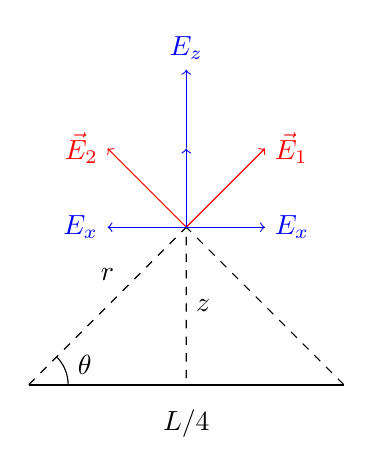
\begin{tikzpicture}
            \draw[thick] (-2,0) -- (2,0);
            \node[below] at (0,-0.2) {$L/4$};
            \draw[dashed] (-2,0) -- (0,2) -- (0,0);
            \draw[dashed] (2,0) -- (0,2);
            \draw[->,red] (0,2) -- (1,3);
            \draw[->,red] (0,2) -- (-1,3);
            \draw[->,blue] (0,3) -- (0,4);
            \draw[->,blue] (0,2) -- (0,3);
            \draw[->,blue] (0,2) -- (1,2);
            \draw[->,blue] (0,2) -- (-1,2);
            \node[red, right] at (1,3) {$\vec{E}_1$};
            \node[red, left] at (-1,3) {$\vec{E}_2$};
            \node[blue, above] at (0,4) {$E_z$};
            \node[blue, right] at (1,2) {$E_x$};
            \node[blue, left] at (-1,2) {$E_x$};
            \node[right] at (0,1) {$z$};
            \node[above] at (-1,1.2) {$r$};
            \draw (-2,0) ++(0:0.5) arc (0:45:0.5);
            \node[right] at (-1.5, 0.25) {$\theta$};
        \end{tikzpicture}
        \end{center}
    \begin{align*}
        &\vec{E}_\text{total}=4E_z\hat{z}\\
        &E_z=\frac{2k\lambda a}{r\sqrt{a^2/4+r^2}}\sin\theta\\
        &r=\sqrt{a^2/4+z^2}\\
        &\sin\theta=\frac{z}{r}\\
        &E_z=\frac{2k\lambda az}{r^2\sqrt{a^2/4+r^2}}\\
        &r^2=\frac{a^2}{4}+z^2\\
        &E_z=\frac{2k\lambda az}{(a^2/4+z^2)\sqrt{a^2/2+z^2}}\\
        &a=\frac{L}{4},\quad\lambda=\frac{Q}{L}\\
        &E_z=\frac{\frac{1}{2}kQ z}{(L^2/64+z^2)\sqrt{L^2/32+z^2}}\\
        &\vec{E}_\text{total}=4E_z\hat{z}=\frac{2kQ z}{(L^2/64+z^2)\sqrt{L^2/32+z^2}}\hat{z}\\
    \end{align*}
    Now we can plug in the values $L=0.16\units{m}$, $Q=40\units{\mu C}$, and $z=0.2\units{m}$ to get the magnitude of the electric field.
    \begin{align*}
        &\vec{E}_\text{total}=\frac{2(8.99\times10^9\units{N\cdot m^2/C^2})(40\times10^{-6}\units{C})(0.2\units{m})}{(0.16^2\units{m^2}/64+(0.2\units{m})^2)\sqrt{(0.16^2\units{m^2}/32+(0.2\units{m})^2)}}\hat{z}=1.76\times10^7\units{N/C}\hat{z}\\
    \end{align*}
    \item The force can be computed as $\vec{F}=q\vec{E}$ and the direction will be toward the center of the square for a negative point charge.
    \begin{align*}
        &\vec{F}=q\vec{E}=-\frac{2kQq z}{(L^2/64+z^2)\sqrt{L^2/32+z^2}}\hat{z}=-88\units{N}\hat{z}\\
    \end{align*}
    \begin{center}
        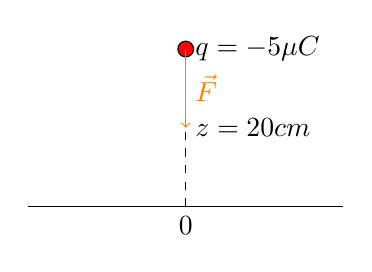
\begin{tikzpicture}
            \draw (-2,0) -- (2,0) node[midway, below] {0};
            \draw[dashed] (0,0) -- (0,2) node[midway, right] {$z=20\units{cm}$};
            \draw[fill=red] (0,2) circle (0.1) node[above, right] {$q=-5\units{\mu C}$};
            \draw[orange, ->] (0,2) -- (0,1) node[midway, right] {$\vec{F}$};
        \end{tikzpicture}
        \end{center}
    \item We can get an expression for the acceleration from the force
    \begin{align*}
        &\vec{F}=m\vec{a}\\
        &\vec{a}=-\frac{2kQq z}{m(L^2/64+z^2)\sqrt{L^2/32+z^2}}\hat{z}\\
    \end{align*}
    \begin{center}
    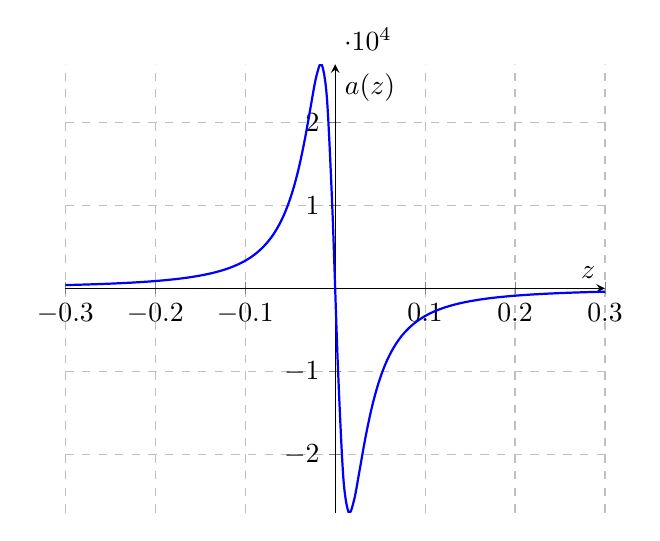
\begin{tikzpicture}
        \begin{axis}[
            axis lines=middle,
            xlabel={$z$},
            ylabel={$a(z)$},
            xmin=-0.3, xmax=0.3,
            % ymin=-2.5, ymax=2.5,
            grid,
            grid style={dashed, gray!50},
            samples=100,
            smooth,
            domain=-0.3:0.3,
        ]
        \addplot[blue,thick] {-2*8.99*10^9*40*10^(-12)*5*x/(0.1*(0.16^2/64+x^2)*sqrt(0.16^2/32+x^2))};
        \end{axis}
    \end{tikzpicture}
    \end{center}
\end{enumerate}
}{}
